
\begin{SCfigure}[0.5][h]
	\centering
	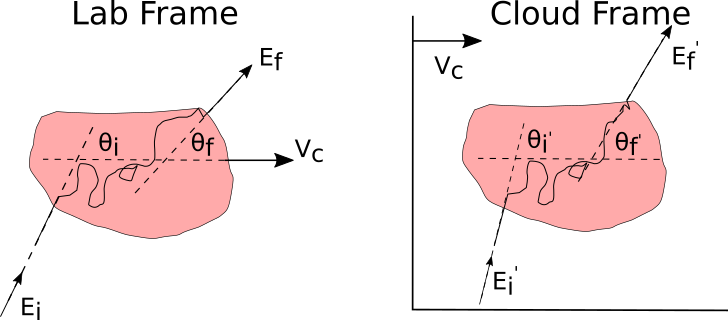
\includegraphics[width=0.7\textwidth]{A1_Supernova_Remnants/Images/fermi_original_theory_frames.png}
	\caption{(\textit{Left})A ISM cloud travelling with velocity $v_\text{cloud}$. A cosmic ray with energy $E_i$ enters the cloud and scatters due to magnetic irregularities. The cosmic ray then leaves the cloud with energy $E_f$. (\textit{Right}) The lorentz transformation into a reference frame where the ISM cloud is at rest.}
	\label{fig:appendix_A_fermi_original_theory_frames}
\end{SCfigure}

As a cosmic ray travels through the interstellar medium, it may encounter an ISM cloud travelling at velocity ($\approx 15~\kmpersec$). Upon entering the ISM cloud, the cosmic ray will scatter due to the magnetic irregularities inside the cloud and leave the cloud with, on average, higher energy. In the reference frame of the cloud (see \autoref{fig:appendix_A_fermi_original_theory_frames}, the scattering of the cosmic ray is collision-less, i.e. no physical interaction. Collisionless interactions are elastic, so in the reference frame of the cloud, the cosmic ray has the same energy before and after scattering. The cosmic ray can undergo multiple scattering events resulting in the outgoing direction to be randomised. Using these conditions and Lorentz transformations, the average energy gain can be calculated in the labatory frame. The general Lorentz transformation of the momentum 4-vector $(\frac{E}{c},\vec{p})$ is:

\begin{equation}
    \begin{aligned}
    E'&=\gamma\qty(E-\beta p_\parallel c) \\
	p_\parallel ' c&=\gamma\qty(p_\parallel c-\beta E) \\
    \end{aligned}
\end{equation}
\noindent where $p_\parallel=p\cos\theta$ is the momentum parallel to the direction of transformation and $p_\perp=p\sin\theta$ is the momentum perpendicular to the direction of transformation. For ultra relativistic particles, $E\approx pc$. Therefore the Lorentz transformation of energy becomes:

\begin{equation}
    \begin{aligned}
    E'&=\gamma\qty(E-\beta pc\cos\theta ) \\
&=\gamma E\qty(1-\beta \cos\theta ) 
    \end{aligned}
\end{equation}
\noindent Therefore the transformation of energy from the lab frame to the clouds reference frame becomes:

\begin{equation}
    \begin{aligned}
    E_1'&=\gamma_\text{cloud}E_1\qty(1-\beta_\text{cloud}\cos\theta_1)
    \end{aligned}
\end{equation}
\noindent where $\beta_\text{cloud}=v_\text{cloud}/c$ is the beta factor for the cloud and $\gamma=1/\sqrt{1-\beta^2}$. As described above, the scattering is elastic in the clouds reference frame. Therefore:

\begin{equation}
    \begin{aligned}
    E_2'&=E_1' \\
&=\gamma_\text{cloud}E_1\qty(1-\beta_\text{cloud}\cos\theta_1)
    \end{aligned}
\end{equation}
\noindent In the laboratory frame (see \autoref{fig:appendix_A_fermi_original_theory_frames}):

\begin{equation}
    \begin{aligned}
    E_2&=\gamma_\text{cloud}E_2'\qty(1--\beta_\text{cloud}\cos\theta_2') \\
&=\gamma_\text{cloud}^2E_1\qty(1+\beta_\text{cloud}\cos\theta_2')\qty(1-\beta_\text{cloud}\cos\theta_1)
    \end{aligned}
\end{equation}

The fractional change in energy becomes:

\begin{equation}
    \begin{aligned}
    \frac{\Delta E}{E}&=\frac{E_2-E_1}{E_1} \\
&=\frac{E_1\qty(1-\beta_\text{cloud}\cos\theta_1+\beta_\text{cloud}\cos\theta_2'-\beta_\text{cloud}^2\cos\theta_1\cos\theta_2')}{E_1\qty(1-\beta_\text{cloud}^2)}-1 \\
&=\frac{1-\beta_\text{cloud}\cos\theta_1+\beta_\text{cloud}\cos\theta_2'-\beta_\text{cloud}^2\cos\theta_1\cos\theta_2'}{1-\beta_\text{cloud}^2}-1
    \end{aligned} \label{eq:appendix_A_fermi_orig_fractional_change_ind}
\end{equation}

\autoref{eq:appendix_A_fermi_orig_fractional_change_ind} shows that head-on collisions (collisions where the cosmic ray and cloud have velocities in the opposite direction) results in energy gain whilst tail collisions (where the cosmic ray and cloud have velocities in the same direction) result in energy loss. The average fractional change of energy is simply:

\begin{equation}
    \begin{aligned}
    \expectation{\frac{\Delta E}{E}}
	&=\frac{1-\beta_\text{cloud}\expectation{\cos\theta_1}+\beta_\text{cloud}\expectation{\cos\theta_2'}-\beta_\text{cloud}^2\expectation{\cos\theta_1}\expectation{\cos\theta_2'}}{1-\beta_\text{cloud}^2}-1
    \end{aligned} \label{eq:appendix_A_fermi_orig_fractional_change_av}
\end{equation}

\noindent where $\expectation\cos\theta_{1,2}$ is the average angle that cosmic rays enter/exit the ISM cloud. In the clouds reference frame, the outgoing direction of the cosmic ray is randomised, therefore $\expectation{\cos\theta_2'}=0$.

\begin{SCfigure}[0.5][hbpt]
	\centering
    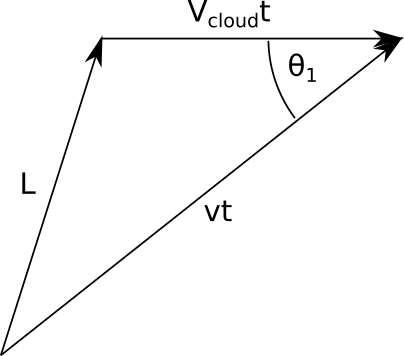
\includegraphics[width=0.5\textwidth]{A1_Supernova_Remnants/Images/fermi_1_collision_rate.png}
	\caption{An interstellar medium cloud at speed $V_\text{cloud}$ is bombarded with cosmic rays travelling at speed $v$.}
	\label{fig:appendix_A_fermi_cloud}
\end{SCfigure}

As shown in \autoref{fig:appendix_A_fermi_cloud} an interstellar medium cloud travels at speed $V_\text{cloud}$ while cosmic rays travel at speed $v$. In time $t$ all cosmic rays along $L$ will have hit the ISM cloud as it travelled distance $V_\text{cloud}t$. Assuming $V_\text{cloud}\ll v$:

\begin{equation}
    \begin{aligned}
    L&=t\sqrt{v^2+V_\text{cloud}^2-2vV_\text{cloud}\cos\theta_1} \\
&\approx \qty(v-V_\text{cloud}\cos\theta_1)t
    \end{aligned}
\end{equation}

\noindent The collision rate of cosmic rays is defined to be:

\begin{equation}
    \begin{aligned}
    R&=n_{CR}\frac{L\sigma}{t} \\
	&=n_{CR}\sigma\qty(v-V_\text{cloud}\cos\theta_1)
    \end{aligned}
\end{equation}

\noindent where $n_{CR}$ is the cosmic ray number density and $\sigma=\pi r^2$ is the cross section of a spherical cloud with radius $r$. Assuming an isotropic distribution of cosmic rays, the fraction of particles between $\theta_1$ and $\theta+\dd{\theta_1}$ is:

\begin{equation}
    \begin{aligned}
        \dv{n_\text{CR}}{\theta_1}&=\frac{n_\text{CR}}{2}\sin\theta \\
        \dv{n_\text{CR}}{\cos\theta_1}&=\frac{n_\text{CR}}{2}
    \end{aligned}
\end{equation}
\noindent where $\ang{0}<\theta<\ang{180}$. The collision rate becomes:
 
\begin{equation}
    \begin{aligned}
    R&=\frac{n_{CR}}{2}\sigma\int_{-1}^{1}\qty(v-V_\text{Cloud}\cos\theta_1)\dd{\cos\theta_1}
    \end{aligned}
\end{equation}


For ultra-relativistic particles ($v\rightarrow c$), the probability distribution of $\cos\theta_1$:

\begin{equation}
    \begin{aligned}
    p_\text{coll}\propto \qty(1-\beta\cos\theta_1),\qquad\qty(-1<\cos\theta_1<1)
    \end{aligned}
\end{equation}

The average value of $\cos\theta_1$ is:

\begin{equation}
    \begin{aligned}
    \expectation{\cos\theta_1}&=\frac{\int_{-1}^{1}\cos\theta_1p_\text{coll}\dd{\cos\theta_1}}{\int_{-1}^{1}p_\text{coll}\dd{\cos\theta_1}} \\
	&=\frac{\int_{-1}^{1}\cos\theta_1\qty(1-\beta\cos\theta_1)\dd{\cos\theta_1}}{\int_{-1}^{1}\qty(1-\beta\cos\theta_1)\dd{\cos\theta_1}} \\
	&=-\frac{\beta_\text{cloud}}{3} 
    \end{aligned} \label{eq:appendix_A_fermi_or_av_theta1}
\end{equation} 

As $\beta_\text{cloud}\ll 1$, combining \autoref{eq:appendix_A_fermi_orig_fractional_change_av} and \autoref{eq:appendix_A_fermi_or_av_theta1}:

\begin{equation}
    \begin{aligned}
    \expectation{\frac{\Delta E}{E}}
	&=\frac{1+\frac{\beta_\text{cloud}^2}{3}}{1-\beta_\text{cloud}}-1 \\
	&\approx\frac{4}{3}\beta_\text{cloud}^2
    \end{aligned} \label{eq:appendix_A_fermi_orig_fractional_change_av_2}
\end{equation}

As $\beta_\text{cloud}\ll 1$, the number of head of collisions is approximately equal to the amount of tail collisions in the lab frame assuming that the cosmic ray distribution is isotropic. Hence, the energy gain is small.

\section{Fermi's second theory of cosmic ray acceleration}

\begin{figure} [h]
	\centering
	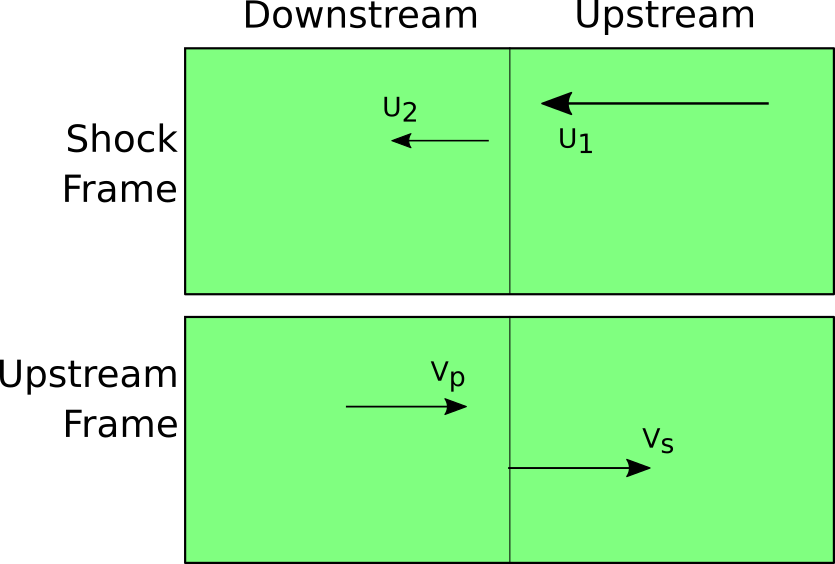
\includegraphics[width=0.7\textwidth]{A1_Supernova_Remnants/Images/fermi_second_theory_frames.png}
	\caption{Propagation of a shock wave (e.g. generated by a supernova remnant) in the reference frame of the shock (\textit{top}) and reference frame of the material `upstream' of the shock (\textit{bottom}). Upstream of the shock represents the region of the ISM that has yet to be "shocked" while downstream references the ISM region that has been "shocked". The shock is represented by the vertical line. In the shock frame, the velocity of the material upstream and downstream of the shock travels at at $U_1=V_s=$ velocity of the shock and $U_2$ respectively. In the upstream reference frame, the shock travels at speed $V_s$ and the ISM clouds downstream travel at velocities $V_p$}
	\label{fig:appendix_A_fermi_2nd_frames}
\end{figure}

Fermi's second theory of cosmic ray acceleration considers cosmic-ray acceleration as a result of shocks and is also known as diffusive shock acceleration. Possible shocks that can accelerate cosmic rays include those in supernova remnants, shocks produced by massive stars in stellar clusters and the extreme environments of active galactic nuclei \citep{2002cra..book.....S}. In the context of this thesis, the forward and reverse shock of supernova remnants will be considered (see \autoref{fig:A1_SNR_Evolution}).
\par~\par
In the reference frame of the material upstream of the shock (the region that has not been `shocked'), the shock travels at velocity $V_s$. After being `shocked', the gas then travels at speed $V_p$. In the reference frame of the shock, the material upstream and downstream of the shock travels at speed $U_1=V_s$ and $U_2$ respectively. The compression value relates the densities of the `shocked' ($\rho_2$) and unshocked' ISM ($\rho_1$).

\begin{equation}
    \begin{aligned}
    R&=\frac{\rho_2}{\rho_1}
    \end{aligned} \label{eq:A1_compression_ratio}
\end{equation}

\noindent By conservation of mass flux:

\begin{equation}
    \begin{aligned}
    \rho_2U_2&=\rho_1U_1=G \\
    \end{aligned} \label{eq:A1_mass_flux_ratio}
\end{equation}

\noindent where $G$ is conserved. For a fluid with specific volume $V$, then $G=U/V$ and \citep{2002cra..book.....S}:

\begin{equation}
    \begin{aligned}
        \frac{V_2}{V_1}&=\frac{\qty(\gamma+1)P_1+\qty(\gamma-1)P_2}{\qty(\gamma-1)P_1+\qty(\gamma+1)P_2} 
    \end{aligned} \label{eq:A1_specific_volume_ratio}
\end{equation}

\noindent with $P$  being the pressure of the gas and $\gamma\approx 5/3$ is the ratio of specific heats upstream and down stream of the shock. Combining \autoref{eq:A1_compression_ratio}, \autoref{eq:A1_mass_flux_ratio} and \autoref{eq:A1_specific_volume_ratio}:

\begin{equation}
    \begin{aligned}
        R&=\frac{GV_1}{GV_2} \\
        &=\frac{\qty(\gamma-1)P_1+\qty(\gamma+1)P_2}{\qty(\gamma+1)P_1+\qty(\gamma-1)P_2}
    \end{aligned}
\end{equation}

By introducing the Alfvenic Mach number, $M$


The velocity downstream of the shock in the shocks reference frame is:

\begin{equation}
    \begin{aligned}
        U_2&=\frac{U_1}{R}=\frac{V_s}{R}
    \end{aligned}
\end{equation}

\noindent In the upstream reference frame, the velocity downstream of the shock is:

\begin{equation}
    \begin{aligned}
        V_P&=V_s-U_2 \\
        &=\frac{V_p-V_s}{R}
    \end{aligned}
\end{equation}

\noindent By conservation of momentum \citep{1983RPPh...46..973D}:

\begin{equation}
    \begin{aligned}
        AU_21=AU_2+P
    \end{aligned}
\end{equation}

\noindent where $P$ is the pressure downstream of the shock. By conservation of energy:

\begin{equation}
    \begin{aligned}
        \frac{1}{2}AU_1^2&=\frac{1}{2}AU_2^2+U_2\qty(E+P) \\
        P\qty(U_1+U_2)&=U_2\qty(E+P) \\
        r&=1+\frac{2E}{P}
    \end{aligned}
\end{equation}

\noindent where $E$ is the downstream internal energy density \citep{1983RPPh...46..973D}. For 
\begin{equation}
    \begin{aligned}
    \frac{V_s}{V_p}&=\frac{R}{R-1}\approx \frac{4}{3}
    \end{aligned}
\end{equation}

Leading to shock velocities in order of $10^4~\kmpersec$.

\subsection{Fractional Energy Gain}

\begin{figure} [h]
	\centering
	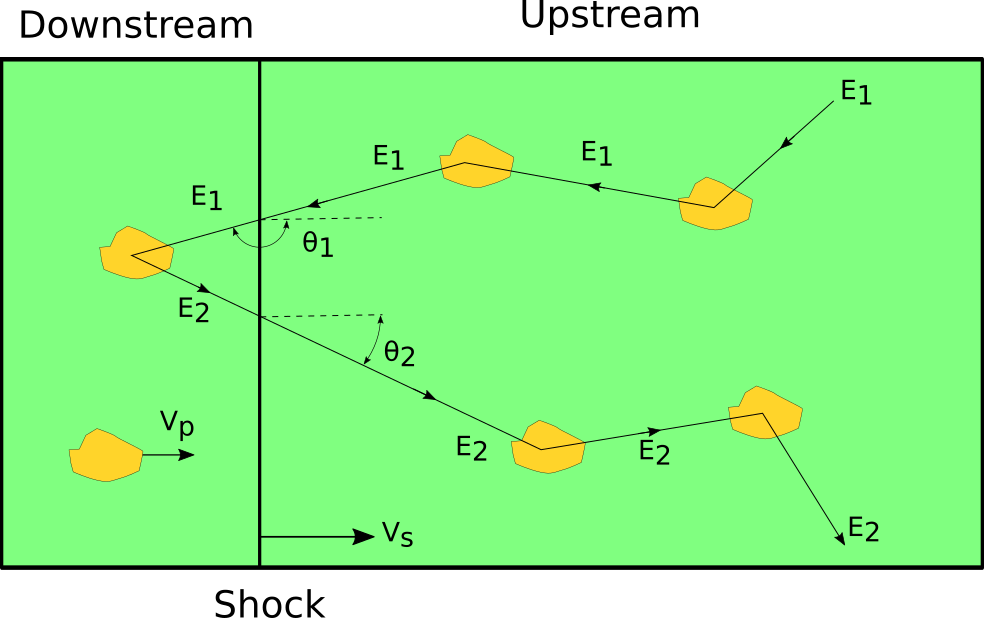
\includegraphics[width=0.7\textwidth]{A1_Supernova_Remnants/Images/fermi_second_theory_clouds.png}
	\caption{In the upstream reference frame. A cosmic ray of energy $E_1$ comes from upstream of the shock and travels through the shock. As it passes through the shock, there is no change of energy. The cosmic ray then scatters of a cloud down stream of the shock and now has energy $E_2$. It passes through the shock again to the upstream region. Now the cosmic ray can either scatter back downstream of the region where it repeats the process, or it can escape and travel out of the system.}
	\label{fig:appendix_A_fermi_2nd_clouds}
\end{figure}

The rate of cosmic rays crossing from upstream to downstream and downstream to upstream is defined by:

\begin{equation}
    \begin{aligned}
    R_{u\rightarrow d}\qty(\theta_1)&\approx-n_{CR}v\cos\theta_1\quad &\si{\per\meter\squared\per\second} \\
R_{d\rightarrow u}\qty(\theta_1)&\approx n_{CR}v\cos\theta_2'\quad&\si{\per\meter\squared\per\second} 
    \end{aligned}
\end{equation}

The probability that a cosmic ray travels upstream to downstream at angle $\theta_1$:

\begin{equation}
    \begin{aligned}
    p\qty(\cos\theta_1)\propto-\cos\theta_1
    \end{aligned}
\end{equation}

giving:

\begin{equation}
    \begin{aligned}
    \expectation{\cos\theta_1}&=\frac{\int_{-1}^{0}\cos\theta_1p_\text{coll}\dd{\cos\theta_1}}{\int_{-1}^{0}p_\text{coll}\dd{\cos\theta_1}} \\
&=-\frac{2}{3}
    \end{aligned} \label{eq:appendix_A_fermi_2nd_theta1_modified}
\end{equation}

and

\begin{equation}
    \begin{aligned}
    p\qty(\cos\theta_2')\propto\cos\theta_2' \\
\expectation{\cos\theta_2'}&=\frac{\int_{-1}^{0}\cos\theta_2'p_\text{coll}\dd{\cos\theta_2'}}{\int_{-1}^{0}p_\text{coll}\dd{\cos\theta_2'}} \\
&=\frac{2}{3}
    \end{aligned} \label{eq:appendix_A_fermi_2nd_theta2_modified}
\end{equation}

combining \autoref{eq:appendix_A_fermi_2nd_theta1_modified} and \autoref{eq:appendix_A_fermi_2nd_theta2_modified} with \autoref{eq:appendix_A_fermi_orig_fractional_change_av_2}:

\begin{equation}
    \begin{aligned}
    \expectation{\frac{\Delta E}{E}}&=\frac{4}{3}\frac{V_p}{c}=\frac{4}{3}\qty(\frac{R-1}{R})\frac{V_s}{c}
    \end{aligned} \label{eq:appendix_A_fermi_2nd_fractional_change}
\end{equation}

where $\beta_p=V_p c\ll 1$. $V_s$ is on order $10^4~\kmpersec$, the fractional energy gain for diffusive shock acceleration is quite higher than for Fermi's original theory of cosmic ray acceleration. Note that Fermi's modified theory of cosmic ray acceleration is first order in $\beta_p$.

\subsection{Probability of escape}

From Fermi's second theory of cosmic ray acceleration, the probability of escape is simply the ratio of the rate of cosmic ray loss downstream to the rate of cosmic rays crossing upstream to downstream:

\begin{equation}
    \begin{aligned}
    \text{Prob}\qty(\text{escape})&=\frac{R_\text{loss}}{R_\text{cross}}
    \end{aligned}
\end{equation}

The rate of cosmic ray loss downstream is the shock speed times the number density of cosmic rays:

\begin{equation}
    \begin{aligned}
    R_\text{loss}&=\frac{n_\text{CR}}{R} V_S~\si{\per\meter\squared\per\second}
    \end{aligned}
\end{equation}

where $R$ is the compression ration. If the rate of cosmic rays travelling upstream to downstream in direction $\cos\theta$ is:

\begin{equation}
    \begin{aligned}
    R_{u\rightarrow d}\qty(\cos\theta) = -n_\text{CR}v\cos\theta
    \end{aligned}
\end{equation}

where $n_\text{CR}$ is the density of cosmic rays and $v$ is the velocity of cosmic ray. The total rate of crossing becomes:

\begin{equation}
    \begin{aligned}
    R_cross&=\frac{1}{4\pi}\int_{-1}^0R_{u\rightarrow d}\qty(\cos\theta_1)2\pi \dd{\cos\theta_1} \\
	&=\frac{-n_\text{CR}v}{2}\int_{-1}^0\cos\theta_1\dd{\cos\theta_1} \\
	&=\frac{n_\text{CR}v}{4}\quad\si{\per\meter\squared\per\second}
    \end{aligned}
\end{equation}

Therefore:

\begin{equation}
    \begin{aligned}
    \text{Prob}\qty(\text{escape})&=\frac{4V_s}{Rv}  
    \end{aligned} \label{eq:appendix_A_prob_escape}
\end{equation}

Notice that the probability that the probability of cosmic ray escaping from the system is not dependent on the cosmic ray number density but rather the velocity of the cosmic ray and the shock wave.

\subsection{Integral Spectrum}

After returning to the shock $k-1$ times, the probability of returning to the shock $k$ times becomes:

\begin{equation}
    \begin{aligned}
    Prob(\text{return })&=\qty[1-\text{Prob}\qty(\text{escape})]^k
    \end{aligned}
\end{equation}

Every time the cosmic ray crosses the shock, it gains energy $\frac{\Delta E}{E}$; therefore after $k$ crossings, the cosmic ray has energy:

\begin{equation}
    \begin{aligned}
    E&=E_0\qty(1+\frac{\Delta}{E})^k
    \end{aligned}
\end{equation}

where $E_0$ is the original cosmic ray energy. This leads to:

\begin{equation}
    \begin{aligned}
    k=\frac{\ln(E/E_0)}{\ln(1+\frac{\Delta E}{E})}
    \end{aligned} \label{eq:appendix_A_k_equation}
\end{equation}

If $N$ is the normalisation constant, the integral spectrum becomes:

\begin{equation}
    \begin{aligned}
    Q\qty(>E)&=N\qty[1-\text{Prob}\qty(\text{escape})]^k
    \end{aligned} \label{eq:appendix_A_integral_spectrum}
\end{equation}

Taking the logarithm of \autoref{eq:appendix_A_integral_spectrum} and combining with \autoref{eq:appendix_A_k_equation}:

\begin{equation}
    \begin{aligned}
    \ln Q\qty(>E)&=A+\frac{\ln(E/E_0)}{\ln(1+\frac{\Delta}{E})}\ln(1-\text{Prob}\qty(\text{escape})) 
    \end{aligned} \label{eq:appendix_A_theoretial_spectrum}
\end{equation}

where $A=\ln N$. The measured power law spectrum has form:

\begin{equation}
    \begin{aligned}
    	Q\qty(>E)&=CE^{-\Gamma}
    \end{aligned}\label{eq:appendix_A_measured_spectrum}
\end{equation}

Taking the natural logarithm of \autoref{eq:appendix_A_measured_spectrum} and equating with \autoref{eq:appendix_A_theoretial_spectrum}:

\begin{equation}
    \begin{aligned}
    \Gamma &= -\frac{\ln(1-\text{Prob}\qty(\text{escape}))}{\ln(1+\frac{\Delta E}{E})}
    \end{aligned}
\end{equation}

Finally substituting in \autoref{eq:appendix_A_fermi_2nd_fractional_change} \& \autoref{eq:appendix_A_prob_escape}:

\begin{equation}
    \begin{aligned}
    \Gamma &=-\frac{\ln(1-\frac{4V_S}{Rv})}{\ln(1+\frac{4}{3}\qty(\frac{R-1}{R})\frac{V_S}{c})}
    \end{aligned}
\end{equation}

Knowing that the speed of the shock is non-relativistic, i.e $V_S\ll c$:

\begin{equation}
    \begin{aligned}
    \Gamma &\approx -\frac{-\frac{4}{R}\frac{V_S}{c}}{\frac{4}{3}\qty(\frac{R-1}{R})\frac{V_S}{c}} \\
% 	&=\frac{3}{R-1}
    \end{aligned}
\end{equation}

Therefore the integral form of the cosmic microwave background becomes:

\begin{equation}
    \begin{aligned}
    Q\qty(>E)\propto E^{-\frac{3}{R-1}}
    \end{aligned}
\end{equation}

and the differential spectrum:

\begin{equation}
    \begin{aligned}
    Q\qty(E)\propto E^{-\frac{R+2}{R-1}}
    \end{aligned}
\end{equation}

For strong shocks $R=4$ leading to $Q\qty(E)\propto E^{-2}$ which is what is approximately measured on Earth.
